% -*-memoria.tex-*-
% Este fichero es parte de la plantilla LaTeX para
% la realización de Proyectos Final de Carrera, protejido
% bajo los términos de la licencia GFDL.
% Para más información, la licencia completa viene incluida en el
% fichero fdl-1.3.tex

% Copyright (C) 2009 Pablo Recio Quijano 

%-------------------------------------------------------
% ---- Plantilla para libros / memorias PFC -----

% Realizada por Pablo Recio Quijano y Noelia Sales Montes 
% Formato de portada y primera página tomado del PFC de
% Francisco Javier Vázquez Púa, en su proyecto 'libgann'
% -------------------------------------------------------

\documentclass[a4paper,11pt]{book}

\usepackage{./estilos/estiloBase} % Basicamente son todas las
                                  % librerias usadas. En caso de que
                                  % falten librerias se van añadiendo
                                  % al fichero.
\usepackage{./estilos/colores}  % Algunos colores ya generados, para
                                % los algunos estilos más avanzados.
\usepackage{./estilos/comandos} % Algunos comandos personalizados

\graphicspath{{./imagenes/}} % Indicamos la ruta donde se encuentran
                             % las imagenes, para ahorrarnos la ruta
                             % completa, y solo modificar aquí si en
                             % un momento dado lo movemos

\begin{document}

% Renombramos las figuras y las tablas
\renewcommand{\figurename}{Figura}
\renewcommand{\listfigurename}{Indice de figuras}
\renewcommand{\tablename}{Tabla}
\renewcommand{\listtablename}{Indice de tablas}

\pagestyle{empty}
% -*-portada.tex-*-
% Este fichero es parte de la plantilla LaTeX para
% la realización de Proyectos Final de Carrera, protejido
% bajo los términos de la licencia GFDL.
% Para más información, la licencia completa viene incluida en el
% fichero fdl-1.3.tex

% Fuente tomada del PFC 'libgann' de Javier Vázquez Púa

\begin{titlepage}

  \begin{center}

    
\includegraphics[scale=0.2]{logo_uca.png} \\
    
    \vspace{2.0cm}
    
    \LARGE{\textbf{ESCUELA SUPERIOR DE INGENIERÍA}} \\
    
    \vspace{1.0cm}
    
    \Large{\textbf{INGENIERÍA TÉCNICA EN INFORMÁTICA DE SISTEMAS}} \\
    
    \vspace{3.0cm}
    
    \Large{ZYCARS: JUEGO DE CONDUCCIÓN 2D} \\
    
    \vspace{2.0cm}
    
    \Large{José Jesús Marente Florín} \\
  
    \vspace{0.5cm}

    \large{\today}
    
  \end{center}
\end{titlepage}

\cleardoublepage

% -*-primerahoja.tex-*-
% Este fichero es parte de la plantilla LaTeX para
% la realización de Proyectos Final de Carrera, protejido
% bajo los términos de la licencia GFDL.
% Para más información, la licencia completa viene incluida en el
% fichero fdl-1.3.tex

% Fuente tomada del PFC 'libgann' de Javier Vázquez Púa

\begin{center}

  
\includegraphics[scale=0.2]{logo_uca.png} \\

  \vspace{2.0cm}

  \Large{ESCUELA SUPERIOR DE INGENIERÍA} \\

  \vspace{1.0cm}

  \large{INGENIERO TÉCNICO EN INFORMÁTICA DE SISTEMAS} \\

  \vspace{2.0cm}

  \large{ZYCARS: JUEGO DE CONDUCCIÓN 2D} \\

  \vspace{1.0cm}

\end{center}

\begin{itemize}
\item \large{Departamento: Lenguajes y Sistemas Informáticos}
\item \large{Director del proyecto: Manuel Palomo Duarte y Juan Manuel Dodero Beardo}
\item \large{Autor del proyecto: José Jesús Marente Florín}
\end{itemize}

\vspace{1.0cm}

\begin{flushright}
  \large{Cádiz, \today} \\

  \vspace{2.5cm}

  \large{Fdo: José Jesús Marente Florín}
\end{flushright}

\cleardoublepage
\pagestyle{plain}

\frontmatter % Introducción, índices ...

% -*-previo.tex-*-
% Este fichero es parte de la plantilla LaTeX para
% la realización de Proyectos Final de Carrera, protejido
% bajo los términos de la licencia GFDL.
% Para más información, la licencia completa viene incluida en el
% fichero fdl-1.3.tex

% Copyright (C) 2009 Pablo Recio Quijano 

\section*{Agradecimientos}

Me gustaría dar las gracias a todos esos compañeros que he conocido durante la carrera y me han ayudado
a lo largo la misma y desarrollo de este proyecto. Así como a mi familia, pareja y amigos por todo el apoyo que me han dado. 
También querría dar las gracias al tutor del proyecto Manuel Palomo por el apoyo, supervisión y consejos que me ha dado. 
Por último a David Nieto Rojas que ha realizado todo el diseño gráfico del proyecto.

\cleardoublepage

\section*{Licencia} % Por ejemplo GFDL, aunque puede ser cualquiera

Este documento ha sido liberado bajo Licencia GFDL 1.3 (GNU Free
Documentation License). Se incluyen los términos de la licencia en
inglés al final del mismo.\\

Copyright (c) 2011 José Jesús Marente FLorín.\\

Permission is granted to copy, distribute and/or modify this document under the
terms of the GNU Free Documentation License, Version 1.3 or any later version
published by the Free Software Foundation; with no Invariant Sections, no
Front-Cover Texts, and no Back-Cover Texts. A copy of the license is included in
the section entitled "GNU Free Documentation License".\\

\cleardoublepage

\section*{Notación y formato}

Cuando nos refiramos a un programa o biblioteca en concreto, utilizaremos la
notación:\\

\emph{Python}.\\

Cuando nos refiramos a un fragmento de código, usaremos la notación:

\begin{lstlisting}[style=Python, numbers=none]
print "Hola mundo" 
\end{lstlisting}

Cuando nos refiramos a algún comando introducido en la terminal, usaremos la notación:

\begin{lstlisting}[style=consola, numbers=none]
sudo apt-get install
\end{lstlisting}
%Cuando nos refiramos a un comando, o función de un lenguaje, usaremos
%la notación: \\ \comando{quicksort}.\\

\cleardoublepage

\tableofcontents
\listoffigures
\listoftables

\mainmatter % Contenido en si ...

\chapter{Introducción}
\begin{frame}
    \frametitle{Introducción}

        \begin{block}{Juegos de conducción}
            \begin{itemize}
                \item Objetivo: llegar a la meta
                \item Zonas diferenciadas
                \item Adictivos
                \item Para todo tipo de jugadores
                %\item Cortos tiempos de juego
                \item Variados modos de juego
                \item No pasan de moda
            \end{itemize}
        \end{block}

    \begin{columns}
    
        \column{150px}
        %\begin{center}
                %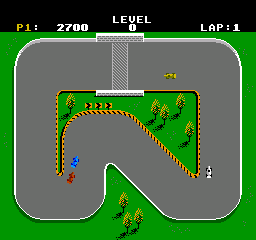
\includegraphics[scale=0.4]{imagenes/super_sprint.png}
        %\end{center}

        \begin{figure}
          \label{logo_latex}
          \begin{center}
            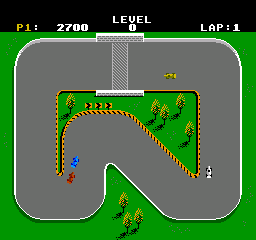
\includegraphics[scale=0.4]{imagenes/super_sprint.png}
          \end{center}
          Super Sprint - Atari (1986)
        \end{figure}
    
        \column{150px}
        \begin{figure}
          \label{logo_latex}
          \begin{center}
            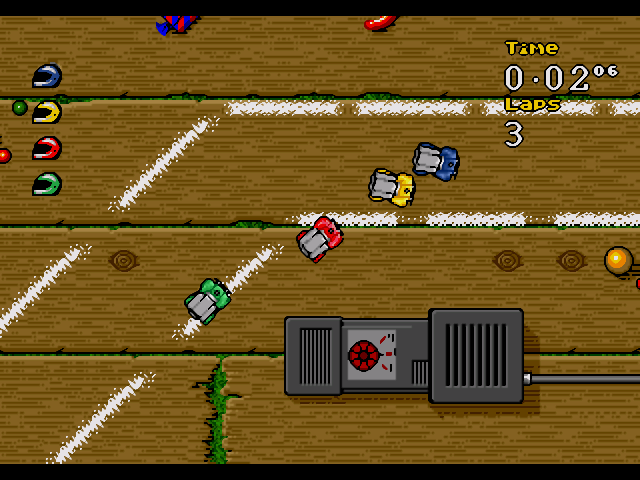
\includegraphics[scale=0.2]{imagenes/micromachines.png}
          \end{center}
          Micromachines - NES (1991)
        \end{figure}

    \end{columns}
    
\end{frame}

\begin{frame}
    \frametitle{Introducción}

    \begin{columns}
    
        \column{150px}
        \begin{block}{Zycars}
            \begin{itemize}
                \item Juego de conducción en 2D con vista cenital
                \item Tres modo de juego
                \item Uso de ítem durante las carreras
            \end{itemize}
        \end{block}

        \column{150px}
        \begin{figure}
          \label{logo_latex}
          \begin{center}
            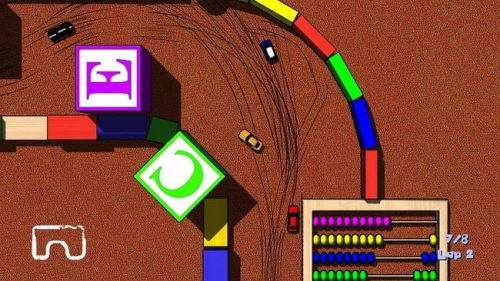
\includegraphics[scale=0.3]{imagenes/toy_cars.jpg}
          \end{center}
          Toy Cars - Xbox 360 (2011)
        \end{figure}
        
    \end{columns}


    \begin{block}{¿Por qué este proyecto?}
        \begin{itemize}
            \item Muy pocos juegos libre con las mismas características
            \item Interés por el mundo de los videojuegos
            \item Cursar la asignatura de Diseño de Videojuegos aumentó el interés por el desarrollo de estos
            \item Contribuir al mundo del software libre
        \end{itemize}
    \end{block}

\end{frame}

\begin{frame}
    \frametitle{Introducción}

    \begin{block}{Objetivos}
        \begin{itemize}
            \item Realizar un juego de coches completamente funcional
            \item Dificultad progresiva (adicción por aprendizaje)
            \item Competidores aceptables, que proponga un desafío superable
            \item Fácilmente ampliable
        \end{itemize}
    \end{block}

    \begin{columns}
    
        \column{200px}
        \begin{alertblock}{No es un simulador}
            \begin{itemize}
                %\item Movimiento básico de los coches
                %\item La colisiones se corrigen de forma sencilla
                \item Arcade, prima la diversión
                \item Coches fáciles de manejar
                \item Colisiones sólo paran a los coches (estrategia)
            \end{itemize}
        \end{alertblock}
        
        \column{100px}
        \begin{figure}
          \label{logo_latex}
          \begin{center}
            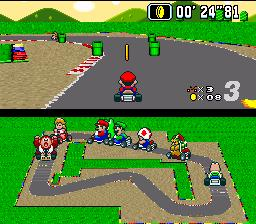
\includegraphics[scale=0.5]{imagenes/super_mario_kart.jpg}
          \end{center}
          Super Mario Kart - SNES (1992)
        \end{figure}
        
    \end{columns}
    
\end{frame}

\clearpage

\chapter{Planificación}
\paragraph{}
La planificación realizada para el desarrollo del proyecto, está dividida en varias partes:

%\begin{itemize}
%    \item \textbf{Fase inicial}: la primera fase consistió en plantear la idea del proyecto, con la ayuda del tutor. Tras varias
%    propuestas realizadas y la deliveración sobre las mismas, se decidió realizar este proyecto.
%    
%    \item \textbf{Fase de análisis}: durante esta etapa se realizó la especificación de los requisitos
%    \item \textbf{}:
%    \item \textbf{}:
%    \item \textbf{}:
%    \item \textbf{}:
%\end{itemize}

\section{Fase inicial}

\paragraph{}
La primera fase consistió en plantear la idea del proyecto, con la ayuda del tutor. Tras varias
propuestas y la deliberación sobre las mismas, se decidió realizar este proyecto.

\paragraph{}
También se pensó en que lenguaje se desarrollaría el proyecto, así como las principales bibliotecas
que se usarían durante la realización del mismo.

\section{Fase de análisis}

\paragraph{}
Esta etapa está dividida principalmente en las dos partes siguiente:

\begin{itemize}
    \item \textbf{Especificación de los requisitos}: estudio de los requisitos que deberá cumplir el juego.
    
    \item \textbf{Recurso necesarios}: recursos necesarios que deberemos usar durante el desarrollo del proyecto.
\end{itemize}

\section{Fase Aprendizaje}

\paragraph{}
Dado que el proyecto se realizaría con un lenguaje de programación del que no se tenían conocimientos, en este caso \emph{Python}, 
así como de la biblioteca que usaríamos en el desarrollo, como es \emph{Pygame}, esta fase se dividió en dos partes:

\begin{itemize}
    \item \textbf{Aprendizaje de \emph{Python}}: periodo empleado para el aprendizaje del lenguaje de programación \emph{Python},
    durante esta etapa se consultó varios libros sobre lenguaje, así como foros de internet y páginas web. Para un aprendizaje más
    ameno y llevadero, se realizaron problemas ya resuelto en otros lenguajes.
    
    \item \textbf{Familiarización con la biblioteca \emph{Pygame}}: tras el periodo de aprendizaje del lenguaje, debía familiarizarme
    con la biblioteca principal que se usaría en el desarrollo del proyecto, como es \emph{Pygame}. Durante su
    aprendizaje se realizaron pequeñas aplicaciones sencillas, para asentar
    bien los conocimientos.
\end{itemize}

\section{Fase de desarrollo}

\paragraph{}
Tras la consecución de las etapas anteriores, se comenzó el desarrollo del proyecto. Esta etapa del desarrollo es la más extensa de 
todas, como es comprensible. Y también la etapa que más subetapas contiene, las principales son la siguientes:

\begin{itemize}
    \item \textbf{Motor básico}: implementación de las necesidades básicas del proyecto, como control del teclado, carga de recursos, movimiento
    de los vehículos.
    
    %\item \textbf{Movimiento de vehículos}: relización del movimiento y comportamiento que deberían tener los vehículos: giro, 
    %aceleración, frenada.
    
    \item \textbf{Carga de escenario}: carga de los circuitos que compondrán el juego de forma que no fuera necesario tocar código
    para la ampliación del juego.
    
    \item \textbf{Creación de menús}: implementación de toda la interfaz de menús de la que estaría compuesto el juego, menú de 
    opciones, selección de personaje, selección de circuito, etc.
    
    \item \textbf{Colisiones}: unos de los aspectos más básico y esenciales de cualquier juego, se debía implementar las colisiones con el
    escenario, así como con otros elementos del juego como pueden ser ítems u otros vehículos.
    
    \item \textbf{Ítems}: implementación del comportamiento y efecto que
    producirían cada uno de los ítems que están disponibles en el juego.
    
    \item \textbf{Inteligencia artificial}: planteamiento y desarrollo de los vehículos que serían manejados por la inteligencia 
    artificial, estos deberían de se capaces de evitar obstáculos, realizar
    recorridos y lanzar ítems.
    
    \item \textbf{Modos de juego}: realización de los modos de juego que componen el proyecto, como serían carrera rápida, contrarreloj
    y campeonato,
\end{itemize}

\section{Pruebas y correcciones}

\paragraph{}
Una de las etapas más importantes, si no es la que más, del desarrollo de cualquier proyecto. Esta etapa se realizaría en paralelo
a la de desarrollo, ya que conforme se implementan nuevas funcionalidades, cada
un debía ser probada exhaustivamente en cualquiera
de las posibles situaciones que pudiera suceder.

\section{Redacción de la memoria}

\paragraph{}
La redacción de la memoria se ha realizado conforme se iba avanzando en el desarrollo del proyecto. Pero tras la finalización
del desarrollo se le ha dedicado más tiempo a la realización de esta.

\section{Diagrama de Gantt}

\paragraph{}
A continuación se muestra la planificación anteriormente comentada, en su correspondiente diagrama de Gantt:

\begin{figure}[H]
  \label{gant1}
  \begin{center}
    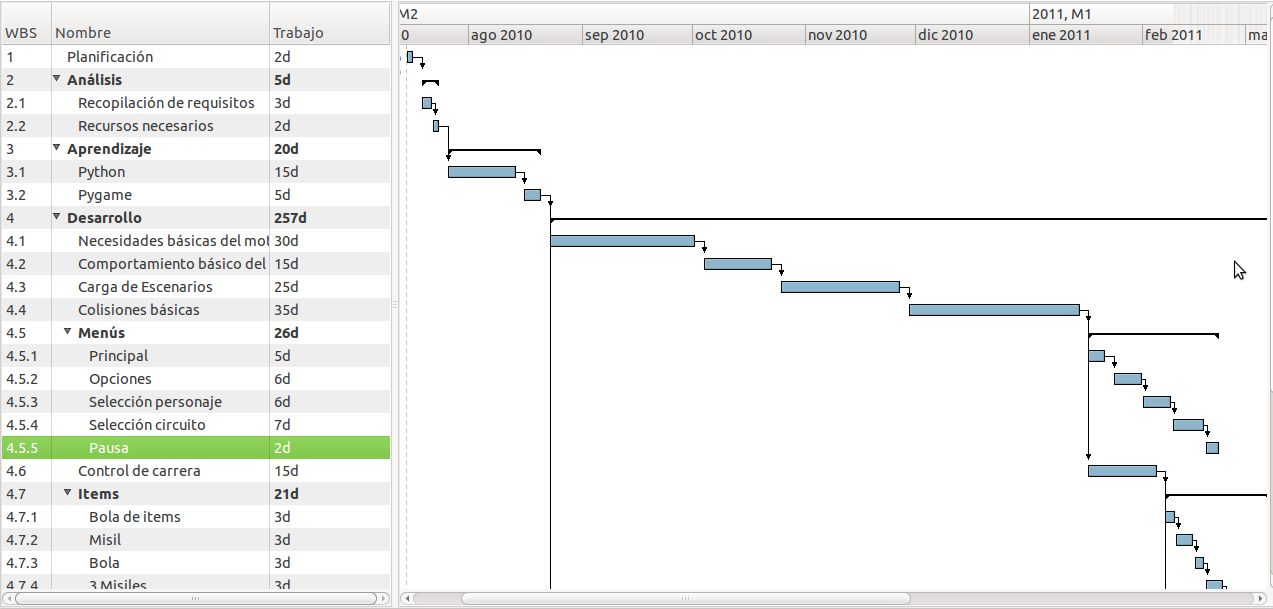
\includegraphics[scale=0.51, angle=90]{imagenes/planificacion/gant1.png}
  \end{center}
  \caption{Planificación: Diagrama de Gantt 1/2.}
\end{figure}

\begin{figure}[H]
  \label{gant2}
  \begin{center}
    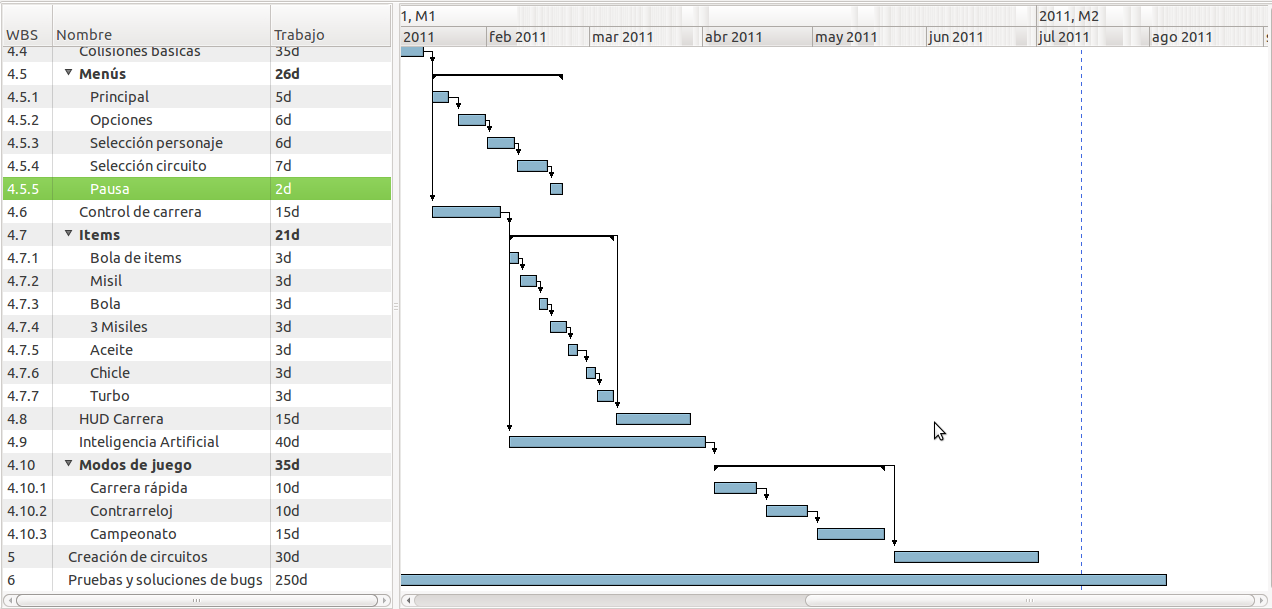
\includegraphics[scale=0.51, angle=90]{imagenes/planificacion/gant2.png}
  \end{center}
  \caption{Planificación: Diagrama de Gantt 2/2.}
\end{figure}

\clearpage

\chapter{Descripción general del proyecto}
%\input{cap2.tex}
\clearpage

\chapter{Análisis}
%\input{cap2.tex}
\clearpage

\chapter{Diseño}
%\input{cap2.tex}
\clearpage

\chapter{Implementación}
\begin{frame}
    \frametitle{Separar datos del código}

        En todo momento se ha procurado separar todos los datos de los personajes, circuitos y menús, del código
        fuente.\\
        \begin{block}{Ventajas}
            \begin{itemize}
                \item No es necesario saber programar para realizar cambios sobre cualquier parámetro.
                \item Cualquier persona puede ampliar el juego con nuevos personajes y nuevos circuitos, siguiendo
                los manuales creados para ello.
            \end{itemize}
        \end{block}
        \begin{block}{Solución}
            \begin{itemize}
                \item Todo se lee de ficheros XML
            \end{itemize}
        \end{block}

\end{frame}

\begin{frame}
    \frametitle{Formato de circuitos}

    \begin{block}{Mapas de tiles}
        Tile: imagen cuadrada, rectangular o hexagonal, utilizada para generar imágenes de mayor complejidad.
    \end{block}   
    
    \begin{block}{Editor de mapas: Tiled}
    Proporcionaba todas las necesidades básicas, 
    como una sencilla edición y creación de niveles, así como la gestión de capas,
    para poder poner elementos en el circuito a un nivel superior o inferior.\\
    Para ello se debía crear una imagen con todos los tiles que compondrían un circuito (tileset).\\
    Genera como resultado un XML.
    \end{block}   

    \begin{block}{Inconveniente}
        No permitia indicar de forma sencilla que tiles eran atravesables, colisionables o de cualquier otro tipo.
    \end{block}

\end{frame}

\begin{frame}
    \frametitle{Formato de circuitos}

        \begin{block}{Solución}
        Una imagen extra con las mismas características, donde los tiles sera de un único color, en función del tipo
        que estos sean.
        \end{block}

        \begin{center}
                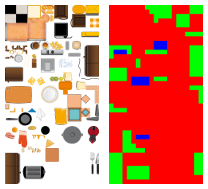
\includegraphics[scale=0.15]{imagenes/tileset-collisionmap.png}
        \end{center}
        

\end{frame}

\begin{frame}
    \frametitle{Colisiones}
    
    Una de las cosas más básicas en cualquier tipo de juego.

    \begin{block}{Colisión con el escenario}
        \begin{itemize}
            \item Detectamos si atravesamos algún tile no atravesable
            \item Si es así corregimos la posición del coche en según la dirección, sentido y lado del tile por
            el que colisione
            \item En el caso de que el tile sea de tipo realentizador, diminuimos la velocidad del coche
        \end{itemize}
    \end{block}

    \begin{center}
        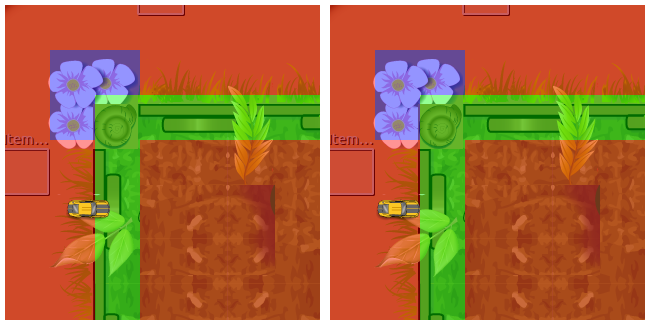
\includegraphics[scale=0.3]{imagenes/colision1-colision2.png}
    \end{center}
\end{frame}

\begin{frame}
    \frametitle{Colisiones}
    
    \begin{block}{Colisión entre vehículos}
        \begin{itemize}
            \item De forma similar a la colisión con el escenario
            \item Cuando se detecta la colisión se corrige la posición de los vehículos, en función la dirección, 
            sentido y lado del tile por el que colisionen
        \end{itemize}
    \end{block}
    
    \begin{block}{Colisión entre vehículos e ítems}
        \begin{itemize}
            \item Si es un ítem de ataque a distancia, destruiremos dicho ítem y cambiaremos el estado del coche con el que
            colisione
            \item Si el ítem es un obstaculo, cambiaremos el estado del coche en función del tipo de ítem
        \end{itemize}
    \end{block}

\end{frame}

\begin{frame}
    \frametitle{Inteligencia artificial}
    Otro de los aspectos más importante de un videojuego de las características de Zycars, es la
    inteligencia artificial, ya que en dos de los tres modos de juegos disponibles el objetivo es obtener la
    mejor clasificación posible, por delante de los demás coches controlados por el ordenador

        \begin{block}{Habilidades}
            \begin{itemize}
                \item Realización del recorrido: debe ser capaz de realizar los 
                recorridos de los circuitos.
                \item Lanzamiento de ítems: también debe poder usar los ítems que reciba de las bolas de ítems.
            \end{itemize}
        \end{block}
\end{frame}

\begin{frame}
    \frametitle{Realización del recorrido. Algoritmo A*}

    Aprovechando que tenemos un circuito creado por tiles y que podemos saber en todo momento en el tile 
    actual que se puede encontrar cualquiera de los competidores, se decidió implementar el 
    algoritmo de búsqueda A*.

        \begin{block}{Objetivo}
        Buscar el camino más corto y óptimo, en el caso de que exista, desde
        un nodo origen, hasta un nodo destino. A la hora de buscar dicho camino se tienen en cuenta factores
        como, el valor heurístico que poseen cada uno de los nodos, así como el coste real del recorrido.
        \end{block}

        \begin{block}{Parámetros}
        Los parametros que se tienen en cuenta en cada uno de los nodos.
            \begin{itemize}
                \item h’(n) es el valor heurístico del nodo actual n, hasta el final
                \item g(n) el coste real del camino desde el origen al nodo actual
                \item Función de evaluación: f(n) = g(n) + h’(n)
            \end{itemize}
        \end{block}

\end{frame}

\begin{frame}
    \frametitle{Realización del recorrido. Algoritmo A*}

        \begin{block}{Estructuras diferenciadas}
            \begin{itemize}
                \item Lista de abiertos: nodos por los que aún no se han pasado
                \item Lista de cerrados: nodos por los que ya se han pasado
            \end{itemize}
        \end{block}

        \begin{block}{Funcionamiento}
            Partiendo de un nodo en el que nos encontramos actualmente:
            \begin{enumerate}
                \item Obtenemos vecinos
                \item Comprobamos que no esten en abiertos ni cerrados
                \item Si alguno esta en abiertos, comprobamos su f(n), si es menor lo sustituiremos
                \item Introducimos en abiertos los que cumplan las condiciones
                \item Obtener de abiertos el nodo que tenga un f(n) menor y comenzamos de nuevo todo el proceso.
                \item Una vez lleguemos al nodo objetivo, detenemos la búsqueda y devolvemos el camino completo.
            \end{enumerate}
        \end{block}

\end{frame}

\begin{frame}
    \frametitle{Realización del recorrido. Algoritmo A*}

        Aplicación en Zycars

        \begin{center}
                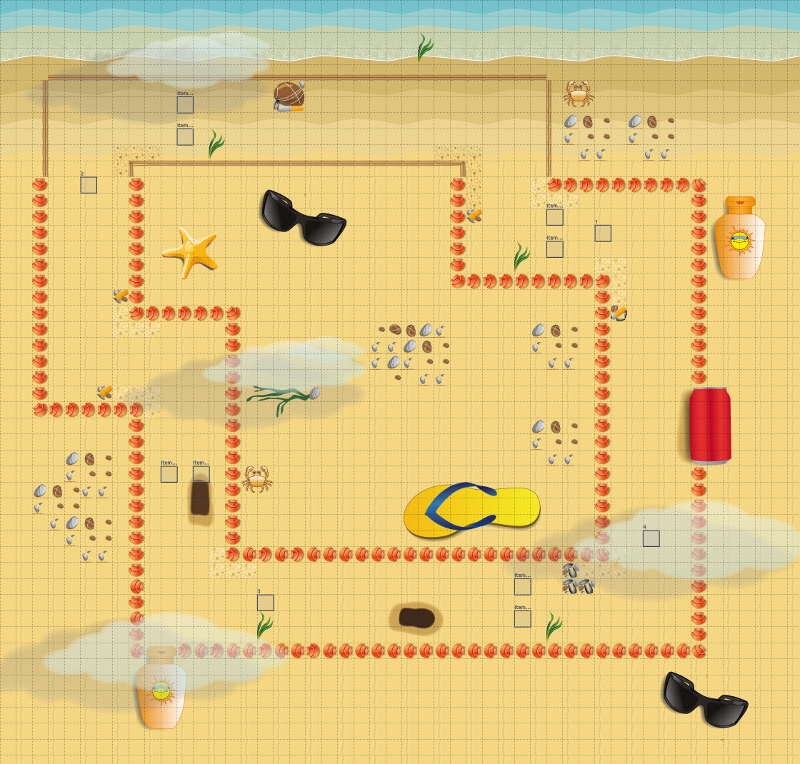
\includegraphics[scale=0.3]{imagenes/ia_check.png}
        \end{center}
        
\end{frame}

\begin{frame}
    \frametitle{Lanzamientos de ítems}

    Capaz de lanzar los ítems disponibles a los largo del juego, según las
    distintas situaciones en la que se encuentre.

        \begin{block}{Solución}
        Se eligió una forma muy sencilla y eficiente a la hora de realizarlo. Para ello cada
        vehículo controlado por la inteligencia artificial, tiene tanto un segmento que va desde el centro del
        coche hacia unos píxeles por delante de la posición actual del vehículo, como otro segmento que
        también va desde el centro pero uno píxeles atrás de la posición del vehículo.
        \end{block}

        \begin{center}
                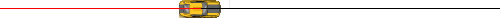
\includegraphics[scale=0.5]{imagenes/ia_segmentos.png}
        \end{center}

\end{frame}

\clearpage

\chapter{Pruebas y validaciones}
%\input{cap2.tex}
\clearpage

\chapter{Conclusiones}
%\input{cap2.tex}
\clearpage

\appendix
\chapter{Manual de instalación}
%%%%%%%%%%%%%%%%%%%%%% WINDOWS %%%%%%%%%%%%%%%%%%%%%%
\section{Windows.}

\paragraph{}
Para jugar a \emph{Zycars} en el sistema operativo Windows no es necesario la instalación de ningún programa
auxiliar, lo único que necesitaremos descargar será la versión correspondiente
a Windows, llamada \textbf{zycars\_1.0\_win.zip } y descomprimirla. La descargaremos
del siguiente enlace:\\

\url{http://code.google.com/p/zycars/downloads/list}

\paragraph{}
Tras descomprimir el archivo, accedemos a la carpeta generada llamada ''zycars\_1.0\_win'' y hacemos doble click 
sobre el archivo \textbf{zycars.exe} para comenzar a jugar.


%%%%%%%%%%%%%%%%%%%%% UBUNTU PAQUETE DEBIAN %%%%%%%%%%%%%%%%%%%%5
\section{Linux: Ubuntu. Desde paquete Debian.}

\paragraph{}
Para poder realizar la instalación de la aplicación desde el paquete Debian, debemos descargarnos el fichero Debian 
llamado \textbf{zycars\_1.0-1\_all.deb}. Descargamos el fichero desde el siguiente enlace:\\

\url{http://code.google.com/p/zycars/downloads/list}

\paragraph{}
Una vez completada la descarga del fichero, hacemos doble click sobre este, y nos indicará si es necesario la instalación 
de algún paquete. Cuando ya estén instaladas todas las dependencias hacemos click en instalar y esperamos a la finalización
de la instalación.

\paragraph{}
Para comenzar a jugar nos vamos a Aplicaciones -> Juegos -> zycars.

\paragraph{}
En el caso que no encontremos el juego instalado en la ruta anterior, lo podremos encontrar en Aplicaciones -> Otras -> zycars.

\paragraph{}
Si por algún motivo no podemos encontrar el enlace directo al juego en las secciones comentadas anteriormente, siempre podremos
abrir una terminar y ejecutar el juego. De la siguiente forma:

\begin{lstlisting}[style=consola, numbers=none]
zycars
\end{lstlisting}

%%%%%%%%%%%%%%%%%%%%%% UBUNTU CÓDIGO FUENTE %%%%%%%%%%%%%%%%%%%%%%
\section{Linux: Ubuntu. Desde código fuente.}

\paragraph{}
Para poder ejecutar \emph{Zycars} desde el código fuente, será necesario la instalación de varias
dependencias, para el correcto funcionamiento de la aplicación.

\paragraph{}
La primera de las dependencias a instalar será \emph{Pygame}, que es la biblioteca principal con la que
se ha desarrollado la aplicación. Para instalar, abrimos una terminal y ejecutamos el siguiente comando:

\begin{lstlisting}[style=consola, numbers=none]
sudo apt-get install python-pygame
\end{lstlisting}

\paragraph{}
Una vez instalado \emph{Pygame}, la siguiente dependencia que instalaremos será \emph{Subversion} para poder
obtener la versión más reciente del proyecto del repositorio del mismo. Para instalar subversion ejecutamos 
la siguiente orden en una terminal:

\begin{lstlisting}[style=consola, numbers=none]
sudo apt-get install subversion
\end{lstlisting}

\paragraph{}
Tras instalar \emph{Subversion}, hacemos checkout del repositorio del proyecto. Para ello ejecutamos en la terminal:

\begin{lstlisting}[style=consola, numbers=none]
svn checkout http://zycars.googlecode.com/svn/trunk/ zycars
\end{lstlisting}

\paragraph{}
Con esto hemos obtenido la versión más reciente del código de la aplicación. Ahora accedemos a la carpeta generada
anteriormente:

\begin{lstlisting}[style=consola, numbers=none]
cd zycars/
\end{lstlisting}

\paragraph{}
Damos permisos de ejecución al fichero principal.

\begin{lstlisting}[style=consola, numbers=none]
chmod +x run_test.py
\end{lstlisting}

\paragraph{}
Tras esto ya podremos jugar sin ningún problema haciendo doble click sobre \textbf{run\_test.py} o ejecutando en la terminal:
\begin{lstlisting}[style=consola, numbers=none]
./run_test.py
\end{lstlisting}


\chapter{Manual de usuario}
%%%%%%%%%%%%%%%%%%%%% MENU PRINCIPAL %%%%%%%%%%%%%%%%%%%%%%%%
\section{Menú principal}

\paragraph{}
Desde el menú principal se podrá acceder a los distintos modos de juego disponibles en \emph{Zycars}, así
como las opciones del juegos y la información sobre los desarrolladores del proyecto.

\begin{figure}[H]
  \label{menu_princiapl}
  \begin{center}
    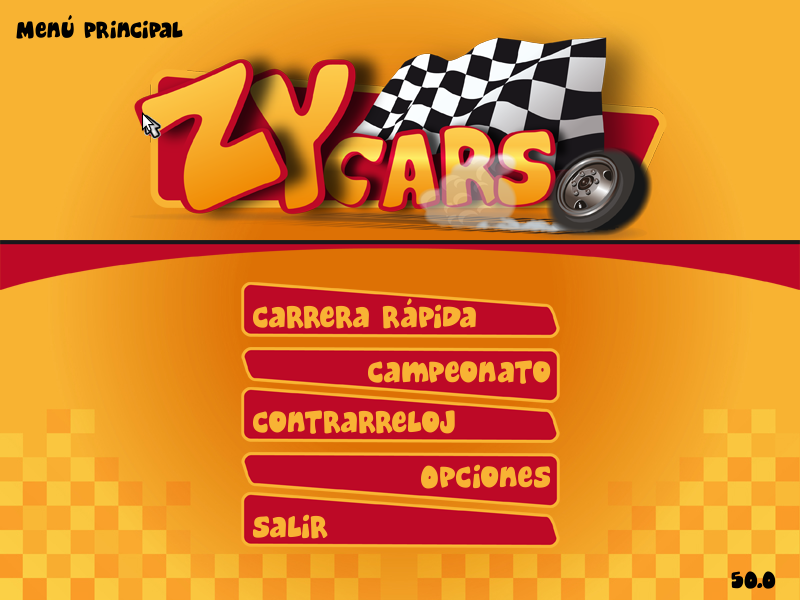
\includegraphics[scale=0.4]{imagenes/capturas/menuprincipal.png}
  \end{center}
  \caption{Manual de usuario: Menú principal}
\end{figure}

\paragraph{}
Debe usar el ratón para seleccionar la opción que desee.

%%%%%%%%%%%%%%%%%%%% MODOS DE JUEGO %%%%%%%%%%%%%%%%%%%%%%%
\section{Modos de juego}

\paragraph{}
En \emph{Zycars} hay disponibles tres modos de juegos, en los que competiremos solos o contra la máquina en función
del objetivo que tengamos que lograr.

\subsection{Carrera rápida}

\paragraph{}
El modo carrera rápida consiste en competir contra la inteligencia artificial en una única carrera, con el objetivo de 
mejorar nuestras habilidades y acostumbrarse a los controles del juego. A lo largo del circuito podremos obtener distintos
ítems con los que hacer frente a nuestros competidores.

\subsection{Campeonato}

\paragraph{}
En el modo Campeonato competiremos contra la inteligencia artificial a lo largo de cuatro circuitos, en los que obtendremos
una puntuación en relación a la posición que hayamos obtenido al concluir la carrera, 4 puntos para el ganador, 2 puntos para
el segundo clasificado, 1 punto para el tercero y 0 puntos para el ultimo en concluir la carrera. El competidor que más puntos haya 
conseguido al concluir el campeonato, será el ganador del mismo. En este modo
también encontraremos ítems durante las distintas carreras.

\subsection{Contrarreloj}

\paragraph{}
En este modo de juego, el modo contrarreloj, el objetivo será batir los
distintos récords de tiempo que tienen cada uno de los 
circuitos, podremos mejorar tanto el tiempo general de la carrera, como el tiempo obtenido en la vuelta más rápida. Tendremos
un máximo de 3 vueltas para mejorar los tiempos. En este modo de juego no
encontraremos ítems, ya que no tendremos ningún oponente
al que tengamos que batir.


%%%%%%%%%%%%%%%%%% SELECCION DE PERSONAJE %%%%%%%%%%%%%%%%%%%%
\section{Menú de selección de personaje}

\paragraph{}
Una vez seleccionado un modo de juego, pasaremos al menú de selección de personaje. En este menú se nos mostrarán todos
los personajes disponibles en \emph{Zycars}, así como el coche que cada uno de ellos conduce y las distintas características
que poseen los coches.

\begin{figure}[H]
  \label{menu_personaje}
  \begin{center}
    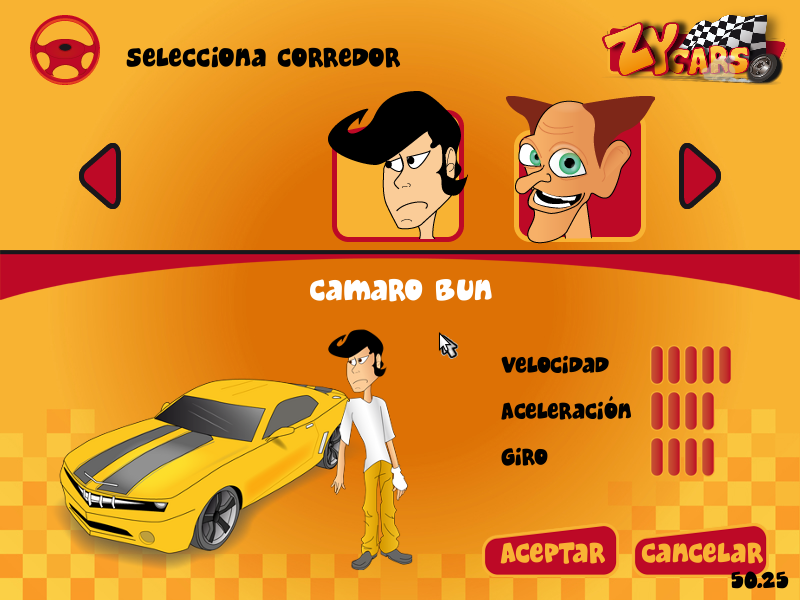
\includegraphics[scale=0.4]{imagenes/capturas/seleccionpersonaje.png}
  \end{center}
  \caption{Manual de usuario: Menú selección de personaje}
\end{figure}

\paragraph{}
Con el ratón podremos navegar sobre los distintos personajes pulsando sobre las flechas rojas. Pulsaremos en el botón
aceptar, para elegir el personaje seleccionado. Si queremos volver al menú principal, pulsaremos sobre el botón cancelar.

%%%%%%%%%%%%%%%%%% SELECCION DE CIRCUITO %%%%%%%%%%%%%%%%%%%%%
\section{Menú de selección de circuito}

\paragraph{}
Una vez seleccionado el personaje con el que deseamos competir, pasaremos al menú de selección de circuito. En este menú
se nos muestran los distintos campeonatos que posee el juego, así como los circuitos que componen cada uno de los 
campeonatos. 

\begin{figure}[H]
  \label{menu_circuito}
  \begin{center}
    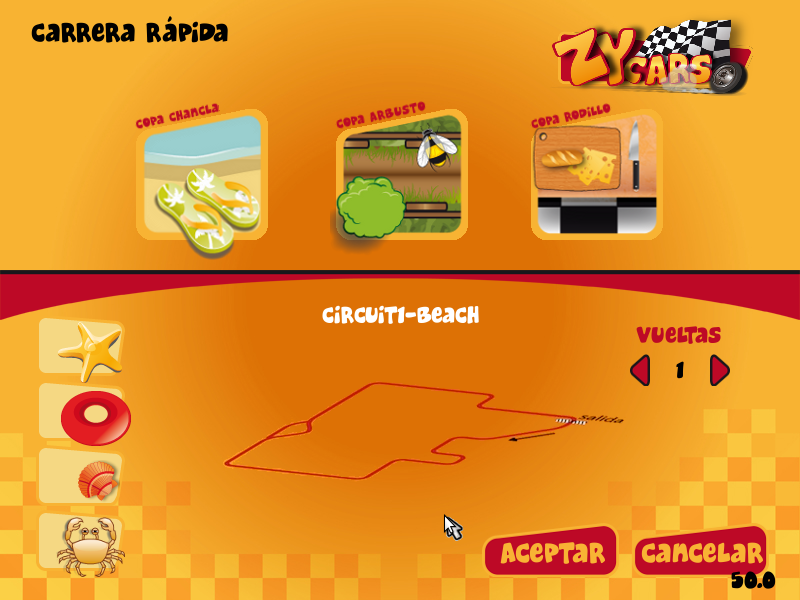
\includegraphics[scale=0.4]{imagenes/capturas/menucircuito.png}
  \end{center}
 \caption{Manual de usuario: Menú selección de circuito}
\end{figure}

\paragraph{}
Si nos encontramos en el modo carrera rápida o en el modo contrarreloj, deberemos seleccionar algún circuito de todos los
disponibles, una vez elegido, pulsaremos aceptar, en el caso de que queramos volver al menú de selección de personaje
pulsaremos sobre el botón cancelar.

\paragraph{}
Si estamos en el modo campeonato, podremos ver todos los circuitos que componen cada uno de los campeonato, al pulsar sobre
el botón aceptar, indicaremos que seleccionamos el campeonato actual. Si pulsamos el botón cancelar volveremos al menú de selección
de personaje.

\paragraph{}
Podremos elegir, en la parte derecha del menú, el número de vueltas que queremos que realicen en cada una de las carreras. Esta opción
no estará disponible en el modo campeonato, ya que en este modo siempre habrá que dar 3 vueltas al circuito.

%%%%%%%%%%%%%%%%%% OPCIONES %%%%%%%%%%%%%%%%%%%%%%
\section{Menú de Opciones}

\paragraph{}
En el menú de opciones, podremos modificar distintos apartados como sonido, características de pantalla y controles del juego. 
Una vez realizados los cambios y deseamos que se apliquen debemos pulsar el botón aceptar, si por el contrario deseamos volver al
menú principal si que se aplique ninguno de los cambios realizados, debemos pulsar sobre el botón cancelar.

\subsection{Sonido}

\paragraph{}
En este menú podremos seleccionar y modificar tanto el volumen de los efectos de sonido que se encuentran en el juego, así 
como el volumen de la música que escuchamos a lo largo de las distintas pantallas y circuitos.

\begin{figure}[H]
  \label{menu_audio}
  \begin{center}
    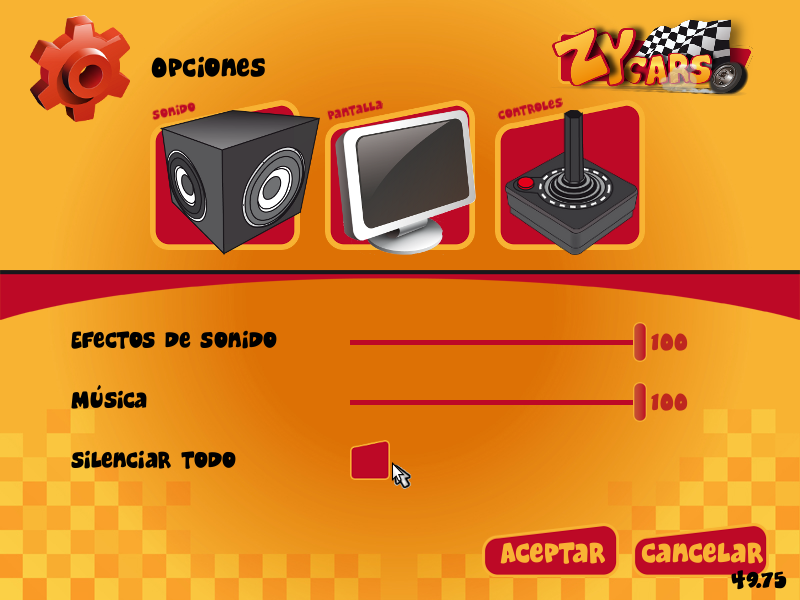
\includegraphics[scale=0.4]{imagenes/capturas/menuopcionesaudio.png}
  \end{center}
 \caption{Manual de usuario: Menú opciones - Audio}
\end{figure}

\paragraph{}
Como podemos ver, hay dos slider para la regulación del sonido y la música. También hay un checkbox, que nos permitirá silenciar todo, tanto 
los efectos de sonido como la música.

\subsection{Pantalla}

\paragraph{}
En este apartado solo dispondremos de una única opción. Esta opción nos
permitirá indicar si deseamos el juego a pantalla 
completa o si por el contrario lo deseamos al tamaño original de 800x600 píxeles.

\begin{figure}[H]
  \label{menu_pantalla}
  \begin{center}
    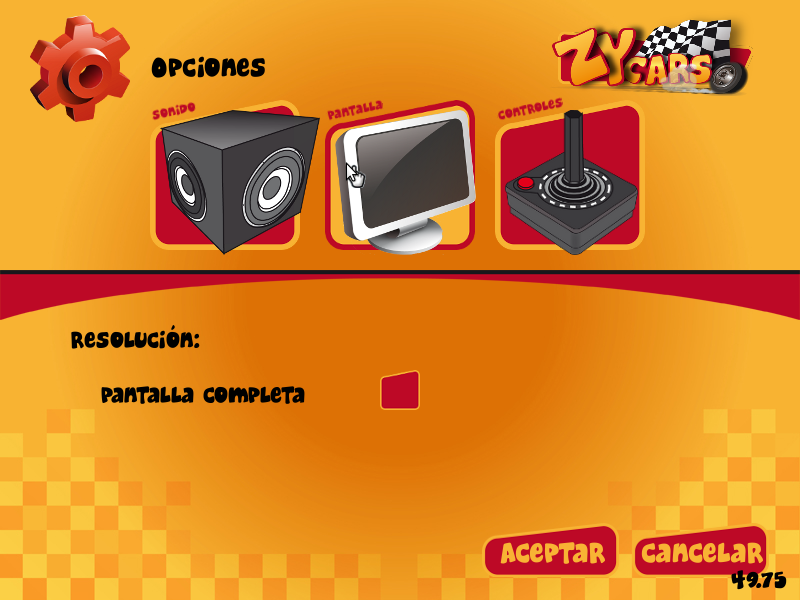
\includegraphics[scale=0.4]{imagenes/capturas/menuopcionespantalla.png}
  \end{center}
 \caption{Manual de usuario: Menú opciones - Pantalla}
\end{figure}

\subsection{Controles}

\paragraph{}
En esta sección del Menú de opciones podemos modificar que controles deseamos a la hora de manejar el vehículo. Los 
controles que podemos modificar son los de dirección, lanzamiento de los ítems y pausar el juego.

\begin{figure}[H]
  \label{menu_controles}
  \begin{center}
    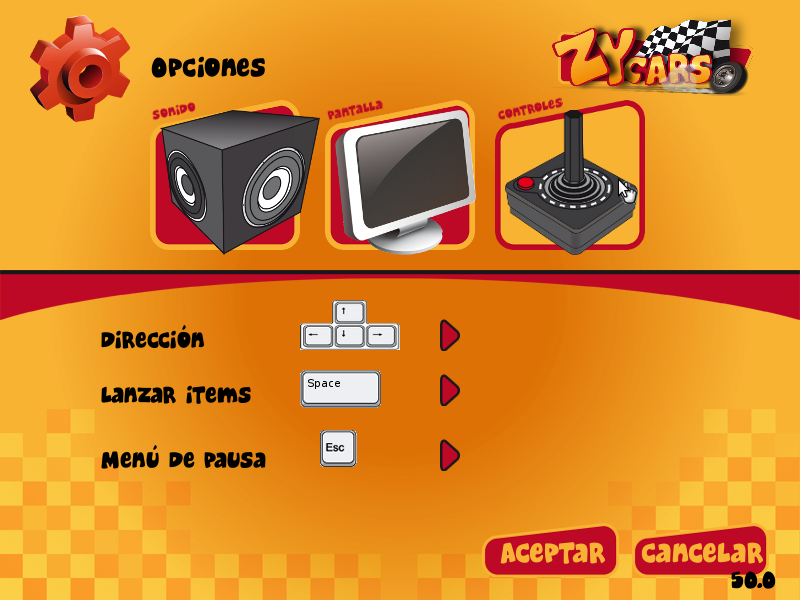
\includegraphics[scale=0.4]{imagenes/capturas/menuopcionescontroles.png}
  \end{center}
 \caption{Manual de usuario: Menú opciones - Controles}
\end{figure}

Debemos pulsar sobre las flechas para modificar los controles que queremos usar.

\section{Ítems}

\paragraph{}
Durante las carreras en las que compitamos contra la máquina, a lo largo de los circuitos encontraremos unas bolas que nos
proporcionarán distintos elementos con los que podremos atacar a nuestros oponentes, dejar obstáculos o aumenten nuestra velocidad
durante un periodo de tiempo.

\begin{figure}[H]
  \label{caja_item}
  \begin{center}
    
\includegraphics[scale=1]{imagenes/items/item_box.png}
  \end{center}
 \caption{Manual de usuario: Bola de ítem.}
\end{figure}

\paragraph{}
Los distintos ítem que podemos conseguir tras atravesar la bola de ítem se describen a continuación:

\begin{itemize}
    \item \textbf{Misil}: este ítem proporciona un único misil al jugador, el cual podremos lanzar a nuestros competidores,
    en caso de que el misil colisione con algún jugador, este perderá el control durante unos instantes. En el caso de que el 
    misil colisione con algún objeto colisionable explotará.
        \begin{figure}[H]
          \label{misil}
          \begin{center}
            
\includegraphics[scale=1]{imagenes/items/missile.png}
          \end{center}
         \caption{Manual de usuario: Misil.}
        \end{figure}
        
    \item \textbf{Misil x 3}: este ítem nos proporciona 3 misiles que tienen las mismas características que el misil normal, 
    introducido anteriormente.
        \begin{figure}[H]
          \label{tres_misiles}
          \begin{center}
            
\includegraphics[scale=1]{imagenes/items/3missile.png}
          \end{center}
         \caption{Manual de usuario: Tres misiles.}
        \end{figure}
        
    \item \textbf{Bola}: este ítem tiene las mismas características que un misil, la única diferencia existente es que al 
    colisionar con algún objete no explotará, si no que rebotará. Sólo explotará en el caso de que colisione con algún
    jugador.        
        \begin{figure}[H]
          \label{bola}
          \begin{center}
            
\includegraphics[scale=1]{imagenes/items/ball.png}
          \end{center}
         \caption{Manual de usuario: Bola.}
        \end{figure}
        
    \item \textbf{Chicle}: este ítem nos proporciona un chicle que al lanzarlo en el circuito, se pegará al asfalto de forma 
    permanente. Cualquier jugador que pase por encima de él, decrementará su velocidad.
        \begin{figure}[H]
          \label{chicle}
          \begin{center}
            
\includegraphics[scale=1]{imagenes/items/gum.png}
          \end{center}
         \caption{Manual de usuario: Chicle.}
        \end{figure}
        
    \item \textbf{Mancha de aceite}: este ítem nos proporciona una mancha de aceite que al lanzarla quedará en el circuito y 
    cualquier jugador que pase por encima, perderá el control del vehículo durante unos instantes.
        \begin{figure}[H]
          \label{mancha_aceite}
          \begin{center}
            
\includegraphics[scale=1]{imagenes/items/oil.png}
          \end{center}
         \caption{Manual de usuario: Macha de aceite.}
        \end{figure}
    
    \item \textbf{Turbo}: este ítem nos permitirá doblar nuestra velocidad durante unos instantes.
        \begin{figure}[H]
          \label{turbo}
          \begin{center}
            
\includegraphics[scale=1]{imagenes/items/turbo.png}
          \end{center}
         \caption{Manual de usuario: Turbo.}
        \end{figure}
        
\end{itemize}



%\blackmatter
%\clearpage

\addcontentsline{toc}{chapter}{Bibliografia y referencias}
\begin{frame}
    \frametitle{Bibliografía recomendada}
    \begin{thebibliography}{5}
        \beamertemplatearticlebibitems
            \bibitem{Python}	
            Página de \emph{Python}
            \newblock http://www.python.org/
            
            \bibitem{PyGTK}
            Página oficial sobre \emph{Pygame}
            \newblock http://www.pygame.org/
             
        \beamertemplatebookbibitems
            \bibitem{UML}
            Larman, Craig
            \newblock Applying UML and Patterns, 3ª Edición. Prentice Hall, 2004.
            
            \bibitem{Dive into Python}
            Pilgrim, Mark
            \newblock Dive into Python. Appress, 2004.
    \end{thebibliography}
\end{frame}

\begin{frame}
    \frametitle{Demostración}
    
    \begin{center}
        {\Huge Demostración de Zycars}
    \end{center}
    
    \begin{center}
        
\includegraphics[scale=0.25]{imagenes/logo_zycars.png}
    \end{center}

\end{frame}

\begin{frame}
    \frametitle{Esto es todo}
    
    \begin{center}
        {\Huge Gracias por su atención}\\
        \bigskip
        {\huge ¿Preguntas?}\\
        \bigskip
        {\LARGE http://code.google.com/p/zycars/}
    \end{center}

\end{frame}


\clearpage
% This is set up to run with pdflatex.
%---------The file header---------------------------------------------
%---------------------------------------------------------------------
\chapter*{\rlap{GNU Free Documentation License}}
\phantomsection  % so hyperref creates bookmarks
\addcontentsline{toc}{chapter}{GNU Free Documentation License}
%\label{label_fdl}

 \begin{center}

       Version 1.3, 3 November 2008


 Copyright \copyright{} 2000, 2001, 2002, 2007, 2008  Free Software Foundation, Inc.
 
 \bigskip
 
     <http://fsf.org/>
  
 \bigskip
 
 Everyone is permitted to copy and distribute verbatim copies
 of this license document, but changing it is not allowed.
\end{center}


\begin{center}
{\bf\large Preamble}
\end{center}

The purpose of this License is to make a manual, textbook, or other
functional and useful document ``free'' in the sense of freedom: to
assure everyone the effective freedom to copy and redistribute it,
with or without modifying it, either commercially or noncommercially.
Secondarily, this License preserves for the author and publisher a way
to get credit for their work, while not being considered responsible
for modifications made by others.

This License is a kind of ``copyleft'', which means that derivative
works of the document must themselves be free in the same sense.  It
complements the GNU General Public License, which is a copyleft
license designed for free software.

We have designed this License in order to use it for manuals for free
software, because free software needs free documentation: a free
program should come with manuals providing the same freedoms that the
software does.  But this License is not limited to software manuals;
it can be used for any textual work, regardless of subject matter or
whether it is published as a printed book.  We recommend this License
principally for works whose purpose is instruction or reference.


\begin{center}
{\Large\bf 1. APPLICABILITY AND DEFINITIONS\par}
\phantomsection
\addcontentsline{toc}{section}{1. APPLICABILITY AND DEFINITIONS}
\end{center}

This License applies to any manual or other work, in any medium, that
contains a notice placed by the copyright holder saying it can be
distributed under the terms of this License.  Such a notice grants a
world-wide, royalty-free license, unlimited in duration, to use that
work under the conditions stated herein.  The ``\textbf{Document}'', below,
refers to any such manual or work.  Any member of the public is a
licensee, and is addressed as ``\textbf{you}''.  You accept the license if you
copy, modify or distribute the work in a way requiring permission
under copyright law.

A ``\textbf{Modified Version}'' of the Document means any work containing the
Document or a portion of it, either copied verbatim, or with
modifications and/or translated into another language.

A ``\textbf{Secondary Section}'' is a named appendix or a front-matter section of
the Document that deals exclusively with the relationship of the
publishers or authors of the Document to the Document's overall subject
(or to related matters) and contains nothing that could fall directly
within that overall subject.  (Thus, if the Document is in part a
textbook of mathematics, a Secondary Section may not explain any
mathematics.)  The relationship could be a matter of historical
connection with the subject or with related matters, or of legal,
commercial, philosophical, ethical or political position regarding
them.

The ``\textbf{Invariant Sections}'' are certain Secondary Sections whose titles
are designated, as being those of Invariant Sections, in the notice
that says that the Document is released under this License.  If a
section does not fit the above definition of Secondary then it is not
allowed to be designated as Invariant.  The Document may contain zero
Invariant Sections.  If the Document does not identify any Invariant
Sections then there are none.

The ``\textbf{Cover Texts}'' are certain short passages of text that are listed,
as Front-Cover Texts or Back-Cover Texts, in the notice that says that
the Document is released under this License.  A Front-Cover Text may
be at most 5 words, and a Back-Cover Text may be at most 25 words.

A ``\textbf{Transparent}'' copy of the Document means a machine-readable copy,
represented in a format whose specification is available to the
general public, that is suitable for revising the document
straightforwardly with generic text editors or (for images composed of
pixels) generic paint programs or (for drawings) some widely available
drawing editor, and that is suitable for input to text formatters or
for automatic translation to a variety of formats suitable for input
to text formatters.  A copy made in an otherwise Transparent file
format whose markup, or absence of markup, has been arranged to thwart
or discourage subsequent modification by readers is not Transparent.
An image format is not Transparent if used for any substantial amount
of text.  A copy that is not ``Transparent'' is called ``\textbf{Opaque}''.

Examples of suitable formats for Transparent copies include plain
ASCII without markup, Texinfo input format, LaTeX input format, SGML
or XML using a publicly available DTD, and standard-conforming simple
HTML, PostScript or PDF designed for human modification.  Examples of
transparent image formats include PNG, XCF and JPG.  Opaque formats
include proprietary formats that can be read and edited only by
proprietary word processors, SGML or XML for which the DTD and/or
processing tools are not generally available, and the
machine-generated HTML, PostScript or PDF produced by some word
processors for output purposes only.

The ``\textbf{Title Page}'' means, for a printed book, the title page itself,
plus such following pages as are needed to hold, legibly, the material
this License requires to appear in the title page.  For works in
formats which do not have any title page as such, ``Title Page'' means
the text near the most prominent appearance of the work's title,
preceding the beginning of the body of the text.

The ``\textbf{publisher}'' means any person or entity that distributes
copies of the Document to the public.

A section ``\textbf{Entitled XYZ}'' means a named subunit of the Document whose
title either is precisely XYZ or contains XYZ in parentheses following
text that translates XYZ in another language.  (Here XYZ stands for a
specific section name mentioned below, such as ``\textbf{Acknowledgements}'',
``\textbf{Dedications}'', ``\textbf{Endorsements}'', or ``\textbf{History}''.)  
To ``\textbf{Preserve the Title}''
of such a section when you modify the Document means that it remains a
section ``Entitled XYZ'' according to this definition.

The Document may include Warranty Disclaimers next to the notice which
states that this License applies to the Document.  These Warranty
Disclaimers are considered to be included by reference in this
License, but only as regards disclaiming warranties: any other
implication that these Warranty Disclaimers may have is void and has
no effect on the meaning of this License.


\begin{center}
{\Large\bf 2. VERBATIM COPYING\par}
\phantomsection
\addcontentsline{toc}{section}{2. VERBATIM COPYING}
\end{center}

You may copy and distribute the Document in any medium, either
commercially or noncommercially, provided that this License, the
copyright notices, and the license notice saying this License applies
to the Document are reproduced in all copies, and that you add no other
conditions whatsoever to those of this License.  You may not use
technical measures to obstruct or control the reading or further
copying of the copies you make or distribute.  However, you may accept
compensation in exchange for copies.  If you distribute a large enough
number of copies you must also follow the conditions in section~3.

You may also lend copies, under the same conditions stated above, and
you may publicly display copies.


\begin{center}
{\Large\bf 3. COPYING IN QUANTITY\par}
\phantomsection
\addcontentsline{toc}{section}{3. COPYING IN QUANTITY}
\end{center}


If you publish printed copies (or copies in media that commonly have
printed covers) of the Document, numbering more than 100, and the
Document's license notice requires Cover Texts, you must enclose the
copies in covers that carry, clearly and legibly, all these Cover
Texts: Front-Cover Texts on the front cover, and Back-Cover Texts on
the back cover.  Both covers must also clearly and legibly identify
you as the publisher of these copies.  The front cover must present
the full title with all words of the title equally prominent and
visible.  You may add other material on the covers in addition.
Copying with changes limited to the covers, as long as they preserve
the title of the Document and satisfy these conditions, can be treated
as verbatim copying in other respects.

If the required texts for either cover are too voluminous to fit
legibly, you should put the first ones listed (as many as fit
reasonably) on the actual cover, and continue the rest onto adjacent
pages.

If you publish or distribute Opaque copies of the Document numbering
more than 100, you must either include a machine-readable Transparent
copy along with each Opaque copy, or state in or with each Opaque copy
a computer-network location from which the general network-using
public has access to download using public-standard network protocols
a complete Transparent copy of the Document, free of added material.
If you use the latter option, you must take reasonably prudent steps,
when you begin distribution of Opaque copies in quantity, to ensure
that this Transparent copy will remain thus accessible at the stated
location until at least one year after the last time you distribute an
Opaque copy (directly or through your agents or retailers) of that
edition to the public.

It is requested, but not required, that you contact the authors of the
Document well before redistributing any large number of copies, to give
them a chance to provide you with an updated version of the Document.


\begin{center}
{\Large\bf 4. MODIFICATIONS\par}
\phantomsection
\addcontentsline{toc}{section}{4. MODIFICATIONS}
\end{center}

You may copy and distribute a Modified Version of the Document under
the conditions of sections 2 and 3 above, provided that you release
the Modified Version under precisely this License, with the Modified
Version filling the role of the Document, thus licensing distribution
and modification of the Modified Version to whoever possesses a copy
of it.  In addition, you must do these things in the Modified Version:

\begin{itemize}
\item[A.] 
   Use in the Title Page (and on the covers, if any) a title distinct
   from that of the Document, and from those of previous versions
   (which should, if there were any, be listed in the History section
   of the Document).  You may use the same title as a previous version
   if the original publisher of that version gives permission.
   
\item[B.]
   List on the Title Page, as authors, one or more persons or entities
   responsible for authorship of the modifications in the Modified
   Version, together with at least five of the principal authors of the
   Document (all of its principal authors, if it has fewer than five),
   unless they release you from this requirement.
   
\item[C.]
   State on the Title page the name of the publisher of the
   Modified Version, as the publisher.
   
\item[D.]
   Preserve all the copyright notices of the Document.
   
\item[E.]
   Add an appropriate copyright notice for your modifications
   adjacent to the other copyright notices.
   
\item[F.]
   Include, immediately after the copyright notices, a license notice
   giving the public permission to use the Modified Version under the
   terms of this License, in the form shown in the Addendum below.
   
\item[G.]
   Preserve in that license notice the full lists of Invariant Sections
   and required Cover Texts given in the Document's license notice.
   
\item[H.]
   Include an unaltered copy of this License.
   
\item[I.]
   Preserve the section Entitled ``History'', Preserve its Title, and add
   to it an item stating at least the title, year, new authors, and
   publisher of the Modified Version as given on the Title Page.  If
   there is no section Entitled ``History'' in the Document, create one
   stating the title, year, authors, and publisher of the Document as
   given on its Title Page, then add an item describing the Modified
   Version as stated in the previous sentence.
   
\item[J.]
   Preserve the network location, if any, given in the Document for
   public access to a Transparent copy of the Document, and likewise
   the network locations given in the Document for previous versions
   it was based on.  These may be placed in the ``History'' section.
   You may omit a network location for a work that was published at
   least four years before the Document itself, or if the original
   publisher of the version it refers to gives permission.
   
\item[K.]
   For any section Entitled ``Acknowledgements'' or ``Dedications'',
   Preserve the Title of the section, and preserve in the section all
   the substance and tone of each of the contributor acknowledgements
   and/or dedications given therein.
   
\item[L.]
   Preserve all the Invariant Sections of the Document,
   unaltered in their text and in their titles.  Section numbers
   or the equivalent are not considered part of the section titles.
   
\item[M.]
   Delete any section Entitled ``Endorsements''.  Such a section
   may not be included in the Modified Version.
   
\item[N.]
   Do not retitle any existing section to be Entitled ``Endorsements''
   or to conflict in title with any Invariant Section.
   
\item[O.]
   Preserve any Warranty Disclaimers.
\end{itemize}

If the Modified Version includes new front-matter sections or
appendices that qualify as Secondary Sections and contain no material
copied from the Document, you may at your option designate some or all
of these sections as invariant.  To do this, add their titles to the
list of Invariant Sections in the Modified Version's license notice.
These titles must be distinct from any other section titles.

You may add a section Entitled ``Endorsements'', provided it contains
nothing but endorsements of your Modified Version by various
parties---for example, statements of peer review or that the text has
been approved by an organization as the authoritative definition of a
standard.

You may add a passage of up to five words as a Front-Cover Text, and a
passage of up to 25 words as a Back-Cover Text, to the end of the list
of Cover Texts in the Modified Version.  Only one passage of
Front-Cover Text and one of Back-Cover Text may be added by (or
through arrangements made by) any one entity.  If the Document already
includes a cover text for the same cover, previously added by you or
by arrangement made by the same entity you are acting on behalf of,
you may not add another; but you may replace the old one, on explicit
permission from the previous publisher that added the old one.

The author(s) and publisher(s) of the Document do not by this License
give permission to use their names for publicity for or to assert or
imply endorsement of any Modified Version.


\begin{center}
{\Large\bf 5. COMBINING DOCUMENTS\par}
\phantomsection
\addcontentsline{toc}{section}{5. COMBINING DOCUMENTS}
\end{center}


You may combine the Document with other documents released under this
License, under the terms defined in section~4 above for modified
versions, provided that you include in the combination all of the
Invariant Sections of all of the original documents, unmodified, and
list them all as Invariant Sections of your combined work in its
license notice, and that you preserve all their Warranty Disclaimers.

The combined work need only contain one copy of this License, and
multiple identical Invariant Sections may be replaced with a single
copy.  If there are multiple Invariant Sections with the same name but
different contents, make the title of each such section unique by
adding at the end of it, in parentheses, the name of the original
author or publisher of that section if known, or else a unique number.
Make the same adjustment to the section titles in the list of
Invariant Sections in the license notice of the combined work.

In the combination, you must combine any sections Entitled ``History''
in the various original documents, forming one section Entitled
``History''; likewise combine any sections Entitled ``Acknowledgements'',
and any sections Entitled ``Dedications''.  You must delete all sections
Entitled ``Endorsements''.

\begin{center}
{\Large\bf 6. COLLECTIONS OF DOCUMENTS\par}
\phantomsection
\addcontentsline{toc}{section}{6. COLLECTIONS OF DOCUMENTS}
\end{center}

You may make a collection consisting of the Document and other documents
released under this License, and replace the individual copies of this
License in the various documents with a single copy that is included in
the collection, provided that you follow the rules of this License for
verbatim copying of each of the documents in all other respects.

You may extract a single document from such a collection, and distribute
it individually under this License, provided you insert a copy of this
License into the extracted document, and follow this License in all
other respects regarding verbatim copying of that document.


\begin{center}
{\Large\bf 7. AGGREGATION WITH INDEPENDENT WORKS\par}
\phantomsection
\addcontentsline{toc}{section}{7. AGGREGATION WITH INDEPENDENT WORKS}
\end{center}


A compilation of the Document or its derivatives with other separate
and independent documents or works, in or on a volume of a storage or
distribution medium, is called an ``aggregate'' if the copyright
resulting from the compilation is not used to limit the legal rights
of the compilation's users beyond what the individual works permit.
When the Document is included in an aggregate, this License does not
apply to the other works in the aggregate which are not themselves
derivative works of the Document.

If the Cover Text requirement of section~3 is applicable to these
copies of the Document, then if the Document is less than one half of
the entire aggregate, the Document's Cover Texts may be placed on
covers that bracket the Document within the aggregate, or the
electronic equivalent of covers if the Document is in electronic form.
Otherwise they must appear on printed covers that bracket the whole
aggregate.


\begin{center}
{\Large\bf 8. TRANSLATION\par}
\phantomsection
\addcontentsline{toc}{section}{8. TRANSLATION}
\end{center}


Translation is considered a kind of modification, so you may
distribute translations of the Document under the terms of section~4.
Replacing Invariant Sections with translations requires special
permission from their copyright holders, but you may include
translations of some or all Invariant Sections in addition to the
original versions of these Invariant Sections.  You may include a
translation of this License, and all the license notices in the
Document, and any Warranty Disclaimers, provided that you also include
the original English version of this License and the original versions
of those notices and disclaimers.  In case of a disagreement between
the translation and the original version of this License or a notice
or disclaimer, the original version will prevail.

If a section in the Document is Entitled ``Acknowledgements'',
``Dedications'', or ``History'', the requirement (section~4) to Preserve
its Title (section~1) will typically require changing the actual
title.


\begin{center}
{\Large\bf 9. TERMINATION\par}
\phantomsection
\addcontentsline{toc}{section}{9. TERMINATION}
\end{center}


You may not copy, modify, sublicense, or distribute the Document
except as expressly provided under this License.  Any attempt
otherwise to copy, modify, sublicense, or distribute it is void, and
will automatically terminate your rights under this License.

However, if you cease all violation of this License, then your license
from a particular copyright holder is reinstated (a) provisionally,
unless and until the copyright holder explicitly and finally
terminates your license, and (b) permanently, if the copyright holder
fails to notify you of the violation by some reasonable means prior to
60 days after the cessation.

Moreover, your license from a particular copyright holder is
reinstated permanently if the copyright holder notifies you of the
violation by some reasonable means, this is the first time you have
received notice of violation of this License (for any work) from that
copyright holder, and you cure the violation prior to 30 days after
your receipt of the notice.

Termination of your rights under this section does not terminate the
licenses of parties who have received copies or rights from you under
this License.  If your rights have been terminated and not permanently
reinstated, receipt of a copy of some or all of the same material does
not give you any rights to use it.


\begin{center}
{\Large\bf 10. FUTURE REVISIONS OF THIS LICENSE\par}
\phantomsection
\addcontentsline{toc}{section}{10. FUTURE REVISIONS OF THIS LICENSE}
\end{center}


The Free Software Foundation may publish new, revised versions
of the GNU Free Documentation License from time to time.  Such new
versions will be similar in spirit to the present version, but may
differ in detail to address new problems or concerns.  See
http://www.gnu.org/copyleft/.

Each version of the License is given a distinguishing version number.
If the Document specifies that a particular numbered version of this
License ``or any later version'' applies to it, you have the option of
following the terms and conditions either of that specified version or
of any later version that has been published (not as a draft) by the
Free Software Foundation.  If the Document does not specify a version
number of this License, you may choose any version ever published (not
as a draft) by the Free Software Foundation.  If the Document
specifies that a proxy can decide which future versions of this
License can be used, that proxy's public statement of acceptance of a
version permanently authorizes you to choose that version for the
Document.


\begin{center}
{\Large\bf 11. RELICENSING\par}
\phantomsection
\addcontentsline{toc}{section}{11. RELICENSING}
\end{center}


``Massive Multiauthor Collaboration Site'' (or ``MMC Site'') means any
World Wide Web server that publishes copyrightable works and also
provides prominent facilities for anybody to edit those works.  A
public wiki that anybody can edit is an example of such a server.  A
``Massive Multiauthor Collaboration'' (or ``MMC'') contained in the
site means any set of copyrightable works thus published on the MMC
site.

``CC-BY-SA'' means the Creative Commons Attribution-Share Alike 3.0
license published by Creative Commons Corporation, a not-for-profit
corporation with a principal place of business in San Francisco,
California, as well as future copyleft versions of that license
published by that same organization.

``Incorporate'' means to publish or republish a Document, in whole or
in part, as part of another Document.

An MMC is ``eligible for relicensing'' if it is licensed under this
License, and if all works that were first published under this License
somewhere other than this MMC, and subsequently incorporated in whole
or in part into the MMC, (1) had no cover texts or invariant sections,
and (2) were thus incorporated prior to November 1, 2008.

The operator of an MMC Site may republish an MMC contained in the site
under CC-BY-SA on the same site at any time before August 1, 2009,
provided the MMC is eligible for relicensing.


\begin{center}
{\Large\bf ADDENDUM: How to use this License for your documents\par}
\phantomsection
\addcontentsline{toc}{section}{ADDENDUM: How to use this License for your documents}
\end{center}

To use this License in a document you have written, include a copy of
the License in the document and put the following copyright and
license notices just after the title page:

\bigskip
\begin{quote}
    Copyright \copyright{}  YEAR  YOUR NAME.
    Permission is granted to copy, distribute and/or modify this document
    under the terms of the GNU Free Documentation License, Version 1.3
    or any later version published by the Free Software Foundation;
    with no Invariant Sections, no Front-Cover Texts, and no Back-Cover Texts.
    A copy of the license is included in the section entitled ``GNU
    Free Documentation License''.
\end{quote}
\bigskip
    
If you have Invariant Sections, Front-Cover Texts and Back-Cover Texts,
replace the ``with \dots\ Texts.'' line with this:

\bigskip
\begin{quote}
    with the Invariant Sections being LIST THEIR TITLES, with the
    Front-Cover Texts being LIST, and with the Back-Cover Texts being LIST.
\end{quote}
\bigskip
    
If you have Invariant Sections without Cover Texts, or some other
combination of the three, merge those two alternatives to suit the
situation.

If your document contains nontrivial examples of program code, we
recommend releasing these examples in parallel under your choice of
free software license, such as the GNU General Public License,
to permit their use in free software.

%---------------------------------------------------------------------


\end{document}
